\documentclass[border=10pt]{standalone}
\usepackage{tikz}
\usetikzlibrary{arrows.meta, positioning, calc, fit, backgrounds}
\usepackage{xcolor}

% Brand colors
\definecolor{Garnet}{HTML}{73000A}
\definecolor{Atlantic}{HTML}{466A9F}
\definecolor{Congaree}{HTML}{1F414D}
\definecolor{Horseshoe}{HTML}{65780B}
\definecolor{Grass}{HTML}{CED318}
\definecolor{Honeycomb}{HTML}{A49137}
\definecolor{Rose}{HTML}{CC2E40}
\definecolor{LightGray}{HTML}{ECECEC}
\definecolor{MedGray}{HTML}{C7C7C7}

\begin{document}
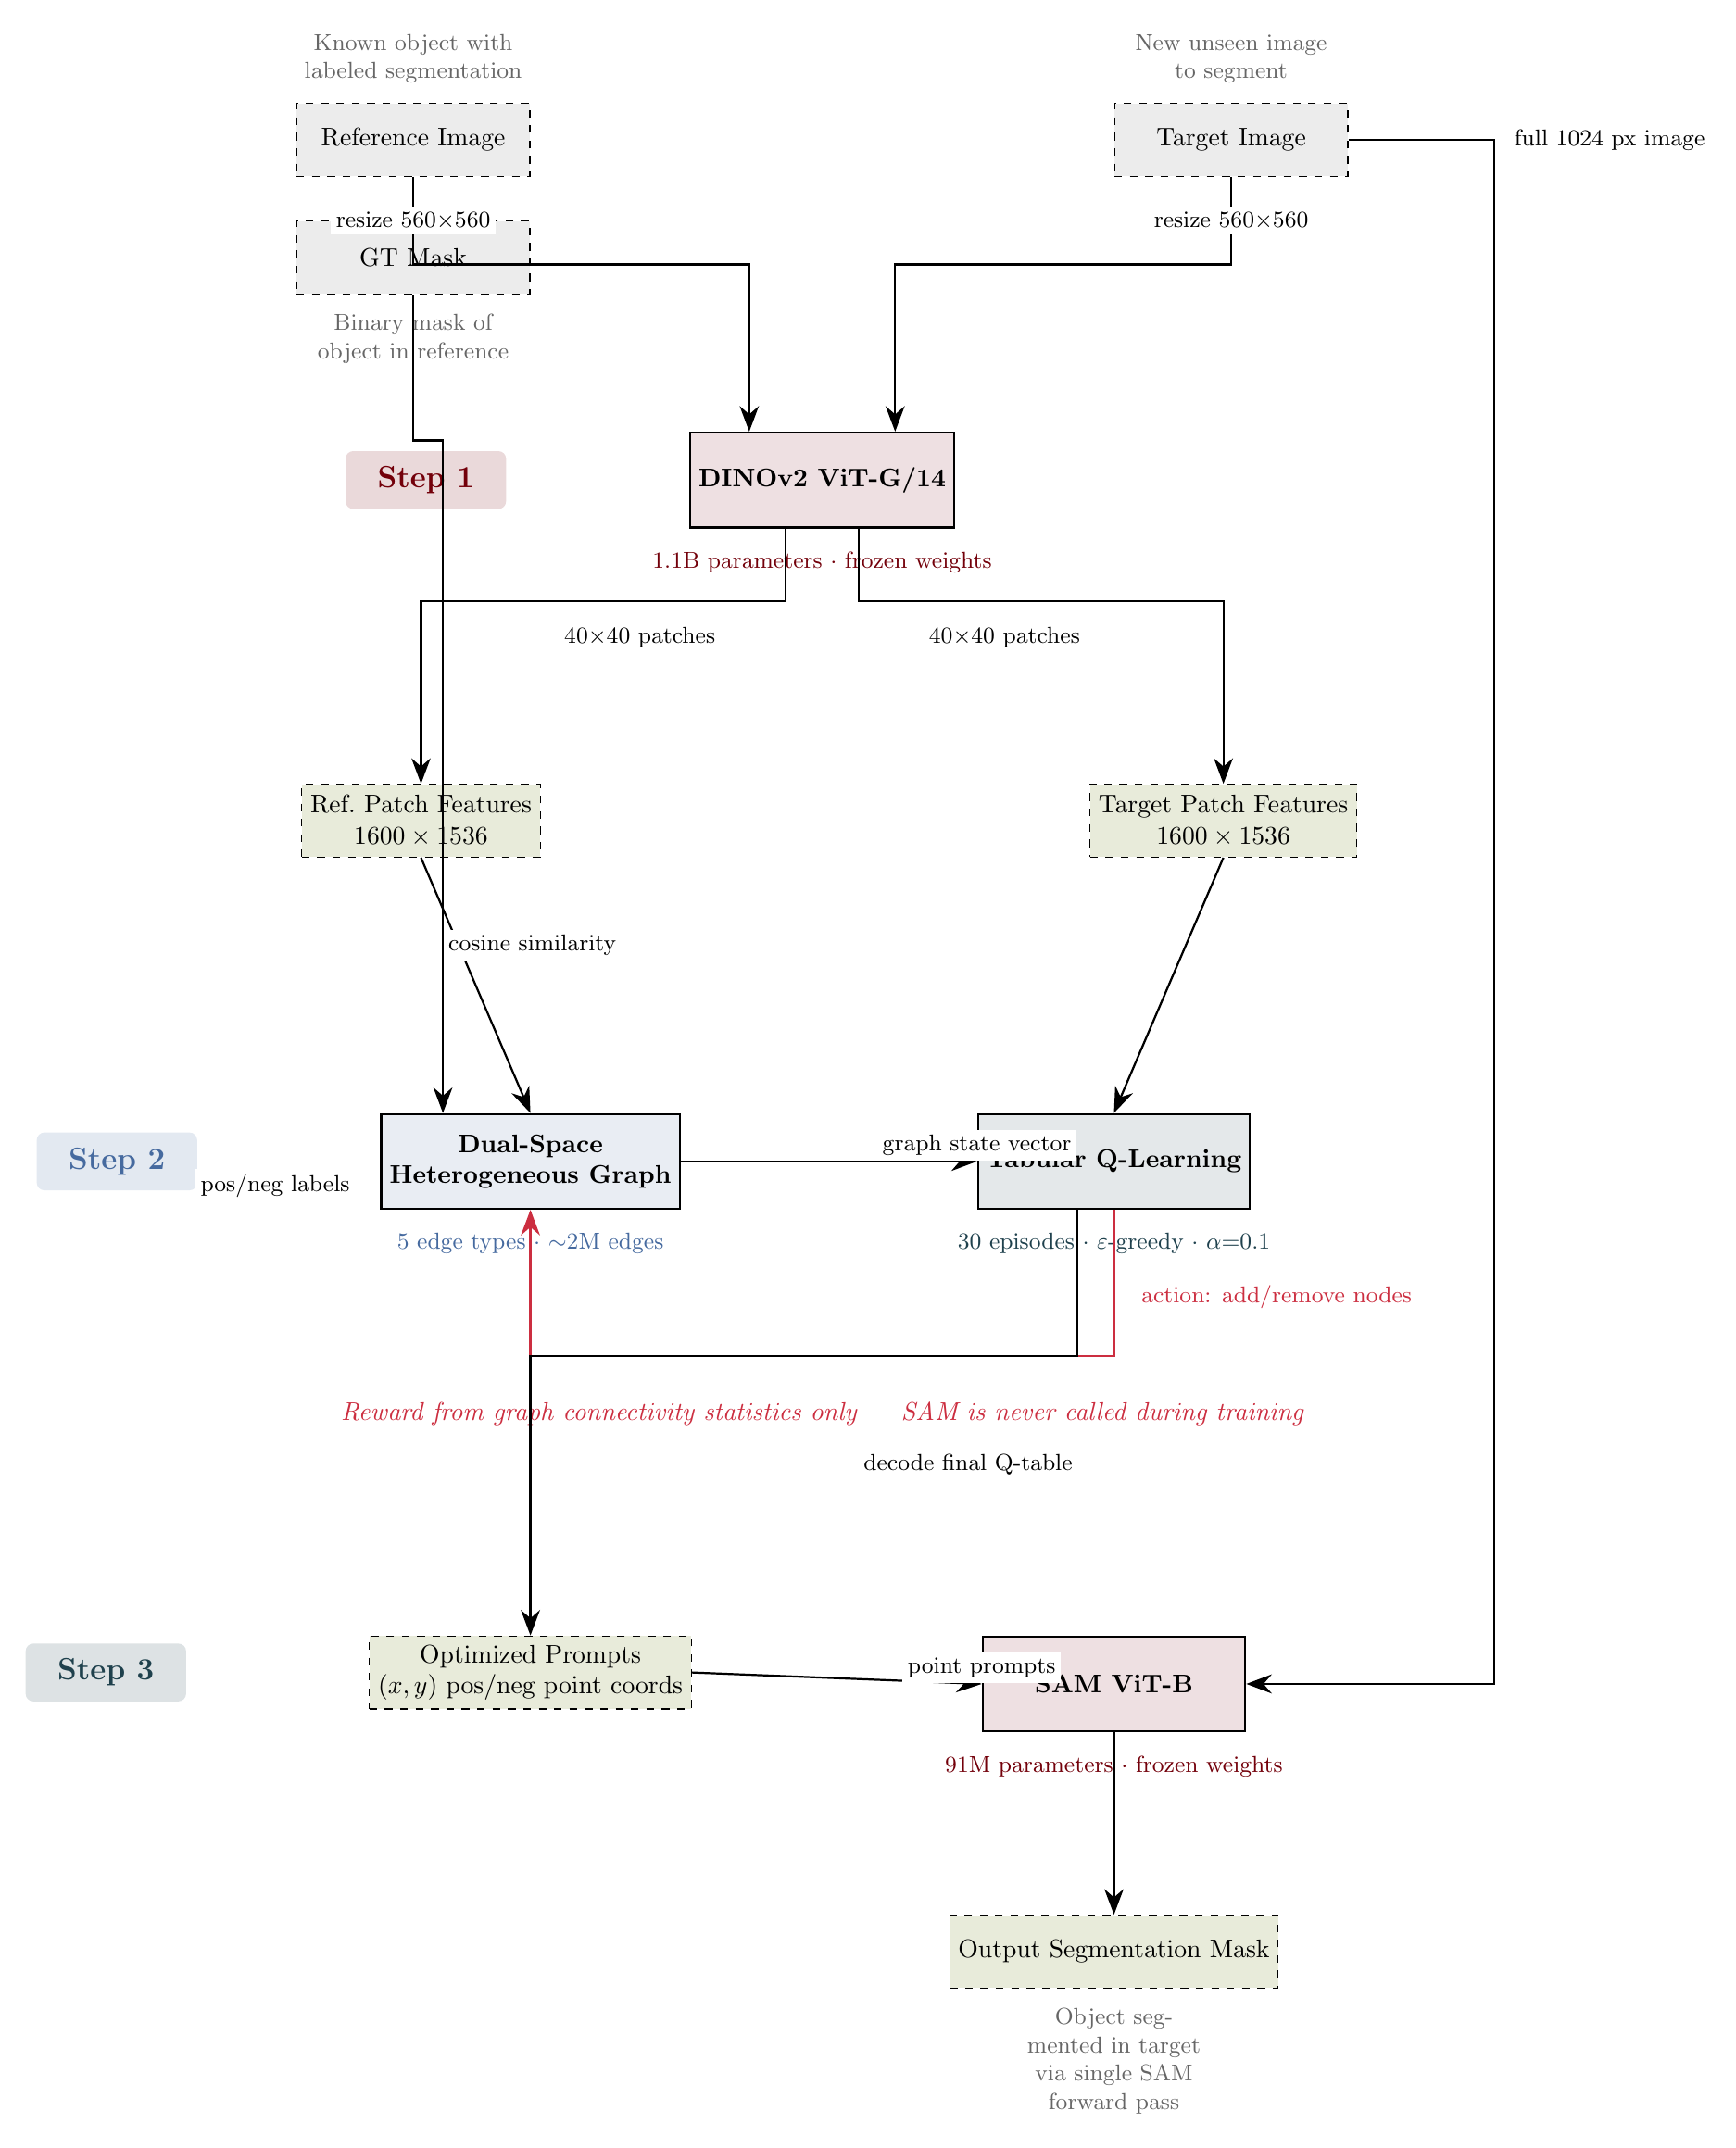
\begin{tikzpicture}[
    model/.style={
        draw, thick, minimum width=3.6cm, minimum height=1.3cm,
        align=center, font=\normalsize\bfseries
    },
    data/.style={
        draw, dashed, minimum width=3.2cm, minimum height=1.0cm,
        align=center, font=\normalsize
    },
    arr/.style={-{Stealth[length=3.5mm]}, thick},
    lbl/.style={font=\small, fill=white, inner sep=2pt},
    desc/.style={font=\small, text width=3.4cm, align=center},
    steplbl/.style={font=\large\bfseries, rounded corners=3pt, inner sep=6pt, minimum width=2.2cm},
    every node/.style={font=\normalsize}
]

% =============================================
% ROW 1: INPUTS
% =============================================
\node[data, fill=LightGray] (ref) {Reference Image};
\node[data, fill=LightGray, below=0.6cm of ref] (gt) {GT Mask};
\node[data, fill=LightGray, right=8.0cm of ref] (target) {Target Image};

\node[desc, above=0.15cm of ref, text=black!60] {Known object with\\labeled segmentation};
\node[desc, above=0.15cm of target, text=black!60] {New unseen image\\to segment};
\node[desc, below=0.15cm of gt, text=black!60] {Binary mask of\\object in reference};

% =============================================
% ROW 2: STEP 1 — DINOv2
% =============================================
\node[model, fill=Garnet!12, below=4.0cm of $(ref)!0.5!(target)$] (dino) {DINOv2 ViT-G/14};
\node[font=\small, below=0.2cm of dino, text=Garnet] {1.1B parameters $\cdot$ frozen weights};

\node[steplbl, fill=Garnet!15, text=Garnet, left=2.5cm of dino] {Step 1};

% Arrows from inputs to DINOv2
\draw[arr] (ref.south) -- ++(0,-1.2) -| ([xshift=-1.0cm]dino.north);
\node[lbl] at ([yshift=-0.6cm]ref.south) {resize $560{\times}560$};

\draw[arr] (target.south) -- ++(0,-1.2) -| ([xshift=1.0cm]dino.north);
\node[lbl] at ([yshift=-0.6cm]target.south) {resize $560{\times}560$};

% =============================================
% ROW 3: FEATURE OUTPUTS (wide spread)
% =============================================
\node[data, fill=Horseshoe!15, below=3.5cm of dino, xshift=-5.5cm] (reffeat) {Ref.\ Patch Features\\$1600 \times 1536$};
\node[data, fill=Horseshoe!15, below=3.5cm of dino, xshift=5.5cm] (tarfeat) {Target Patch Features\\$1600 \times 1536$};

\draw[arr] ([xshift=-0.5cm]dino.south) -- ++(0,-1.0) -| (reffeat.north);
\node[lbl] at ([xshift=-2.5cm, yshift=-1.5cm]dino.south) {40$\times$40 patches};

\draw[arr] ([xshift=0.5cm]dino.south) -- ++(0,-1.0) -| (tarfeat.north);
\node[lbl] at ([xshift=2.5cm, yshift=-1.5cm]dino.south) {40$\times$40 patches};

% =============================================
% ROW 4: STEP 2 — Graph + Q-Learning (wide spread)
% =============================================
\node[model, fill=Atlantic!12, below=3.5cm of reffeat, xshift=1.5cm] (graph) {Dual-Space\\Heterogeneous Graph};
\node[font=\small, below=0.2cm of graph, text=Atlantic] {5 edge types $\cdot$ ${\sim}$2M edges};

\node[model, fill=Congaree!12, below=3.5cm of tarfeat, xshift=-1.5cm] (qlearn) {Tabular Q-Learning};
\node[font=\small, below=0.2cm of qlearn, text=Congaree] {30 episodes $\cdot$ $\varepsilon$-greedy $\cdot$ $\alpha{=}0.1$};

\node[steplbl, fill=Atlantic!15, text=Atlantic,
    left=2.5cm of graph] {Step 2};

% Features into graph
\draw[arr] (reffeat.south) -- (graph.north);
\node[lbl, anchor=west] at ([xshift=0.3cm, yshift=-1.2cm]reffeat.south) {cosine similarity};

\draw[arr] (tarfeat.south) -- (qlearn.north);

% GT mask into graph
\draw[arr] (gt.south) -- ++(0,-2.0) -| ([xshift=-1.2cm]graph.north);
\node[lbl] at ([xshift=-3.5cm, yshift=-1.0cm]graph.north) {pos/neg labels};

% Graph to Q-learning
\draw[arr] (graph.east) -- (qlearn.west)
    node[lbl, above] {graph state vector};

% Q-learning reward loop (more space below)
\draw[arr, Rose, thick] (qlearn.south) -- ++(0,-2.0)
    -| (graph.south);
\node[lbl, text=Rose, anchor=west] at ([xshift=0.3cm, yshift=-1.2cm]qlearn.south)
    {action: add/remove nodes};

\node[font=\normalsize\itshape, text=Rose]
    at ([yshift=-2.8cm]$(graph.south)!0.5!(qlearn.south)$)
    {Reward from graph connectivity statistics only --- SAM is never called during training};

% =============================================
% ROW 5: STEP 3 — Prompt Decoding + SAM (wide spread)
% =============================================
\node[data, fill=Horseshoe!15, below=6.5cm of $(graph)!0.5!(qlearn)$, xshift=-4.0cm] (prompts) {Optimized Prompts\\$(x,y)$ pos/neg point coords};

\node[model, fill=Garnet!12, below=6.5cm of $(graph)!0.5!(qlearn)$, xshift=4.0cm] (sam) {SAM ViT-B};
\node[font=\small, below=0.2cm of sam, text=Garnet] {91M parameters $\cdot$ frozen weights};

\node[steplbl, fill=Congaree!15, text=Congaree,
    left=2.5cm of prompts] {Step 3};

% Q-learning to prompts
\draw[arr] ([xshift=-0.5cm]qlearn.south) -- ++(0,-2.0) -| (prompts.north);
\node[lbl] at ([xshift=-2.0cm, yshift=-3.5cm]qlearn.south) {decode final Q-table};

% Target image to SAM (route along far right side)
\draw[arr] (target.east) -- ++(2.0,0) |- (sam.east);
\node[lbl, anchor=west] at ([xshift=2.2cm]target.east) {full $1024$ px image};

% Prompts to SAM
\draw[arr] (prompts.east) -- (sam.west)
    node[lbl, above] {point prompts};

% =============================================
% ROW 6: OUTPUT
% =============================================
\node[data, fill=Horseshoe!15, below=2.5cm of sam] (mask) {Output Segmentation Mask};
\node[desc, below=0.15cm of mask, text=black!60] {Object segmented in target\\via single SAM forward pass};

\draw[arr] (sam.south) -- (mask.north);

\end{tikzpicture}
\end{document}
